\documentclass[12pt, a4paper]{article}
\usepackage{array} % and/or
\usepackage{longtable} % and/or
\usepackage{colortab} % or
\usepackage{colortbl}
\usepackage{arydshln}
\usepackage{epsfig}
\usepackage{subfigure}
%\usepackage{amscd}
\usepackage{amssymb}
\usepackage{amsbsy}
\usepackage{framed}
\usepackage{amsthm, amsmath}
%\usepackage[dvips]{graphicx}
\usepackage{natbib}
\bibliographystyle{chicago}
\usepackage{vmargin}
% left top textwidth textheight headheight
% headsep footheight footskip
\setmargins{3.0cm}{2.5cm}{15.5 cm}{22cm}{0.5cm}{0cm}{1cm}{1cm}
\renewcommand{\baselinestretch}{1.5}
\pagenumbering{arabic}
\theoremstyle{plain}
\newtheorem{theorem}{Theorem}[section]
\newtheorem{corollary}[theorem]{Corollary}
\newtheorem{ill}[theorem]{Example}
\newtheorem{lemma}[theorem]{Lemma}
\newtheorem{proposition}[theorem]{Proposition}
\newtheorem{conjecture}[theorem]{Conjecture}
\newtheorem{axiom}{Axiom}
\theoremstyle{definition}
\newtheorem{definition}{Definition}[section]
\newtheorem{notation}{Notation}
\theoremstyle{remark}
\newtheorem{remark}{Remark}[section]
\newtheorem{example}{Example}[section]
\renewcommand{\thenotation}{}
\renewcommand{\thetable}{\thesection.\arabic{table}}
\renewcommand{\thefigure}{\thesection.\arabic{figure}}
\author{ } \date{ }


\begin{document}
\tableofcontents
\newpage

\begin{framed}

	\subsubsection*{Types of Variables (Revision)}
	\begin{itemize}
		\item Examples of \textbf{continuous variables} include revision time (measured in hours), intelligence (measured using IQ score), exam performance (measured from 0 to 100), weight (measured in kg), and so forth. 
		
		\item Examples of \textbf{ordinal variables} include \textit{Likert} items (e.g., a 7-point scale from "strongly agree" through to "strongly disagree"), amongst other ways of ranking categories (e.g., a 3-point scale explaining how much a customer liked a product, ranging from "Not very much" to "Yes, a lot"). 
		\item Examples of \textbf{nominal variables} include gender (e.g., 2 groups: male and female), ethnicity (e.g., 3 groups: Caucasian, African American and Hispanic), profession (e.g., 5 groups: surgeon, doctor, nurse, dentist, therapist), and so forth.
	\end{itemize}
\end{framed}
	\newpage
\section*{Introduction to Logistic Regression}

Logistic regression determines the impact of multiple independent variables
presented simultaneously to predict membership of one or other of the two
dependent variable categories.

\section{Binomial Logistic Regression} 
A binomial logistic regression (often referred to simply as logistic regression), predicts the probability that an observation falls into one of two categories of a \textbf{dichotomous} dependent variable based on one or more independent variables that can be either continuous or categorical.

\section{Binomial Logistic Regression: Model Diagnostics}

\begin{itemize}
	\item In order to understand how much variation in the dependent variable can be explained by the model (the equivalent of $R^2$ in multiple regression), you sho$R^2$uld consult Model Summary statistics.
	
	\item The SPSS output table below contains the \textit{Cox \& Snell R Square} and \textit{Nagelkerke R Square }values, which are both methods of calculating the explained variation. These values are sometimes referred to as pseudo $R^2$ values (and will have lower values than in multiple regression).
	\item  However, they are interpreted in the same manner, but with more caution. Therefore, the explained variation in the dependent variable based on our model ranges from 24.0\% to 33.0\%, depending on whether you reference the Cox \& Snell $R^2$ or Nagelkerke $R^2$ methods, respectively. 
	
	\item Nagelkerke $R^2$ is a modification of Cox \& Snell $R^2$, the latter of which cannot achieve a value of 1. For this reason, it is preferable to report the Nagelkerke $R^2$ value.
\end{itemize}
\begin{verbatim}
\begin{figure}[h!]
\centering
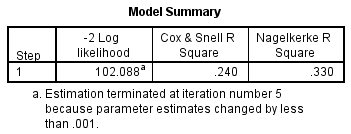
\includegraphics[width=0.9\linewidth]{BLogReg-Rsq}
\caption{SPSS output}
\label{fig:BLogReg-Rsq}
\end{figure}
\end{verbatim}


\section{Binomial Logistic Regression}
Binomial logistic regression estimates the probability of an event (as an example, having heart disease) occurring. 
\begin{itemize}
	\item If the estimated probability of the event occurring is greater than or equal to 0.5 (better than even chance), the procedure classifies the event as occurring (e.g., heart disease being present). \item If the probability is less than 0.5, Logistic regression classifies the event as not occurring (e.g., no heart disease). 
\end{itemize}
\subsection{Category Prediction Table}




It is very common to use binomial logistic regression to predict whether cases can be correctly classified (i.e., predicted) from the independent variables. Therefore, it becomes necessary to have a method to assess the effectiveness of the predicted classification against the actual classification. There are many methods to assess this with their usefulness oftening depending on the nature of the study conducted. However, all methods revolve around the observed and predicted classifications, which are presented in the ``Classification Table", as shown below:

\begin{verbatim}
\begin{figure}[h!]
\centering
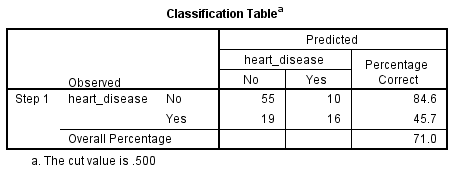
\includegraphics[width=0.97\linewidth]{BLogReg-Table}
\caption{SPSS Output}
\label{fig:BLogReg-Table}
\end{figure}
\end{verbatim}

Firstly, notice that the table has a subscript which states, ``The cut value is .500". This means that if the probability of a case being classified into the "yes" category is greater than .500, then that particular case is classified into the "yes" category. 
Otherwise, the case is classified as in the "no" category. 

\subsection{Interpreting the Classifcation Table}
Whilst the classification table appears to be very simple, it actually provides a lot of important information about your binomial logistic regression result, including:


\begin{itemize}
	\item[A.] The \textbf{percentage accuracy in classification (PAC)}, which reflects the percentage of cases that can be correctly classified as "no" heart disease with the independent variables added (not just the overall model).
	\item[B.] \textbf{Sensitivity}, which is the percentage of cases that had the observed characteristic (e.g., "yes" for heart disease) which were correctly predicted by the model (i.e., true positives).
	\item[C.] \textbf{Specificity}, which is the percentage of cases that did not have the observed characteristic (e.g., "no" for heart disease) and were also correctly predicted as not having the observed characteristic (i.e., true negatives).
	\item[D.] The \textbf{positive predictive value}, which is the percentage of correctly predicted cases "with" the observed characteristic compared to the total number of cases predicted as having the characteristic.
	\item[E.] The \textbf{negative predictive value}, which is the percentage of correctly predicted cases ``without" the observed characteristic compared to the total number of cases predicted as not having the characteristic.
\end{itemize}
%--------------------------------------------------------------------------------------%


\section{Introduction to Logistic Regression}
\begin{itemize}
	\item Logistic regression or logit regression is a type of probabilistic statistical classification model.
	
	\item It is also used to predict a binary response from a binary predictor, used for predicting the outcome of a categorical dependent variable (i.e., a class label) based on one or more predictor variables (features). 
	
	\item That is, it is used in estimating empirical values of the parameters in a qualitative response model. The probabilities describing the possible outcomes of a single trial are modeled, as a function of the explanatory (predictor) variables, using a logistic function. 
	
	\item Logistic regression, also called a logit model, is used to model \textbf{dichotomous (i.e. Binary) outcome variables}. In the logit model the log odds of the outcome is modeled as a linear combination of the predictor variables.
\end{itemize}


\subsection{Examples of Logistic Regression}

\begin{description}
	\item[Example 1:]  Suppose that we are interested in the factors that influence whether a political candidate wins an election.  The outcome (response) variable is binary (0/1); \textit{ win or lose}.  The predictor variables of interest are the amount of money spent on the campaign, the amount of time spent campaigning negatively and whether or not the candidate is an incumbent.
	
	\item[Example 2:]  A researcher is interested in how variables, such as GRE (Graduate Record Exam scores), GPA (grade point average) and prestige of the undergraduate institution, effect admission into graduate school. The response variable, \textit{admit/don't admit}, is a binary variable.
\end{description}

%You could use binomial logistic regression to understand whether exam performance can be predicted based on revision time, test anxiety and lecture attendance (i.e., where the dependent variable is ``exam performance", measured on a dichotomous scale – ``passed" or ``failed" – and you have three independent variables: ``revision time", ``test anxiety" and ``lecture attendance"). 
%
%
%Alternately, you could use binomial logistic regression to understand whether drug use can be predicted based on prior criminal convictions, drug use amongst friends, income, age and gender (i.e., where the dependent variable is ``drug use", measured on a dichotomous scale – ``yes" or ``no" – and you have five independent variables: ``prior criminal convictions", ``drug use amongst friends", ``income", ``age" and "gender").
\newpage
\subsection{Assumptions}

\begin{description}
	\item[Assumption 1:] Your dependent variable should be measured on a \textbf{dichotomous scale}. Examples of dichotomous variables include gender (two groups: "males" and "females"), presence of heart disease (two groups: "yes" and "no"), personality type (two groups: "introversion" or "extroversion"), body composition (two groups: "obese" or "not obese"), and so forth. \\
	\newline
	However, if your dependent variable was not measured on a dichotomous scale, but a continuous scale instead, you will need to carry out \textbf{multiple regression}, whereas if your dependent variable was measured on an ordinal scale, \textbf{ordinal regression} would be a more appropriate starting point.
	
	\item[Assumption 2:] You have one or more independent variables, which can be either continuous (i.e., an interval or ratio variable) or categorical (i.e., an ordinal or nominal variable). 
	
	
	
	\item[Assumption 3:] You should have independence of observations and the dependent variable should have mutually exclusive and exhaustive categories.
	
	\item[Assumption 4:] There needs to be a linear relationship between any continuous independent variables and the logit transformation of the dependent variable. 
\end{description}

%----------------------------------------------------------------------------------------%


\section{Logistic Regression: Odds Ratios and Log-Odds}
\begin{itemize}
	\item Suppose that in a sample of 100 men, 90 drank wine in the previous week, while in a sample of 100 women only 20 drank wine in the same period. \item The odds of a man drinking wine are 90 to 10, or 9:1, while the odds of a woman drinking wine are only 20 to 80, or 1:4 = 0.25:1. 
	\item The odds ratio is thus 9/0.25, or 36, showing that men are much more likely to drink wine than women. 
	\item The detailed calculation is:
	
	
	\[ { 0.9/0.1 \over 0.2/0.8}=\frac{\;0.9\times 0.8\;}{\;0.1\times 0.2\;} ={0.72 \over 0.02} = 36 \]
	
	\item This example also shows how odds ratios are sometimes sensitive in stating relative positions: in this sample men are 90/20 = 4.5 times more likely to have drunk wine than women, but have 36 times the odds. 
	
	
	
	\item The logarithm of the odds ratio, the difference of the logits of the probabilities, tempers this effect, and also makes the measure symmetric with respect to the ordering of groups. 
	\item For example, using natural logarithms, an odds ratio of 36/1 maps to 3.584, and an odds ratio of 1/36 maps to -3.584.
\end{itemize}


\section*{Logistic Regression: Logit Transformation}
%http://data.princeton.edu/wws509/notes/c3.pdf

The logit transformation is given by the following formula: 
\[ \eta_i = \mbox{logit}(\pi_i)  = \mbox{log}\left( \frac{\pi_i}{1- \pi_i} \right) \]

\noindent 
The inverse of the logit transformation is given by the following formula: 
\[ \pi_i = \mbox{logit}^{-1}(\eta_i)  =  \frac{e^{\eta_i}}{1 + e^{\eta_i}} \]

%---------------------------%
\subsection*{Example 1}
Given that $\pi_i = 0.2$, compute $\eta_i$.

\[ \eta_i = \mbox{log}\left( \frac{0.2}{1-0.2} \right)= \mbox{log}\left( \frac{0.2}{0.8} \right)\] 

\[ \eta_i =  \mbox{log}(0.25) =-1.386 \]

%---------------------------%
\subsection*{Example 2}
Given that $\eta_i = 2.3$, compute $\pi_i$.

\[ \pi_i  =  \frac{e^{2.3}}{1 + e^{2.3}} = \frac{9.974}{1 + 9.974} = 0.908 \]

%--------------------------------------------------------------------------------------%

\subsection*{Logits}
In logistic regression, the logit may be computed in a manner similar to linear regression:
\[ \eta_i = \beta_0 + \beta_1x_1 + \beta_2x_2 + \ldots  \]

%---------------------------%

\section{Logistic Regression: Odds Ratios and Log-Odds}
\begin{itemize}
	\item Suppose that in a sample of 100 men, 90 drank wine in the previous week, while in a sample of 100 women only 20 drank wine in the same period. The odds of a man drinking wine are 90 to 10, or 9:1, while the odds of a woman drinking wine are only 20 to 80, or 1:4 = 0.25:1. 
	\item The odds ratio is thus 9/0.25, or 36, showing that men are much more likely to drink wine than women. The detailed calculation is:
	
	\[ { 0.9/0.1 \over 0.2/0.8}=\frac{\;0.9\times 0.8\;}{\;0.1\times 0.2\;} ={0.72 \over 0.02} = 36 \]
	
	\item This example also shows how odds ratios are sometimes sensitive in stating relative positions: in this sample men are 90/20 = 4.5 times more likely to have drunk wine than women, but have 36 times the odds. 
	
	
	\item The logarithm of the odds ratio, the difference of the logits of the probabilities, tempers this effect, and also makes the measure symmetric with respect to the ordering of groups. For example, using natural logarithms, an odds ratio of 36/1 maps to 3.584, and an odds ratio of 1/36 maps to -3.584.
\end{itemize}



\section*{Logistic function} 

The logistic function, with $\beta_0 + \beta_1 x$ on the horizontal axis and $\pi(x)$ on the vertical axis
An explanation of logistic regression begins with an explanation of the logistic function, which always takes on values between zero and one:
\[
F(t) = \frac{e^t}{e^t+1} = \frac{1}{1+e^{-t}},
\]
and viewing t as a linear function of an explanatory variable x (or of a linear combination of explanatory variables), the logistic function can be written as:
\[\pi(x) = \frac{e^{(\beta_0 + \beta_1 x)}} {e^{(\beta_0 + \beta_1 x)} + 1} = \frac {1} {1+e^{-(\beta_0 + \beta_1 x)}}.
\]
This will be interpreted as the probability of the dependent variable equalling a ``success" or ``case" rather than a failure or non-case. We also define the inverse of the logistic function, the logit:
\[g(x) = \ln \frac {\pi(x)} {1 - \pi(x)} = \beta_0 + \beta_1 x ,
\]and equivalently:
\[\frac{\pi(x)} {1 - \pi(x)} = e^{(\beta_0 + \beta_1 x)}.
\]
%======================================================%

\section{Logistic Regression: Logits}
%http://data.princeton.edu/wws509/notes/c3.pdf

The logit transformation is given by the following formula: 
\[ \eta_i = \mbox{logit}(\pi_i)  = \mbox{log}\left( \frac{\pi_i}{1- \pi_i} \right) \]

To inverse of the logit transformation is given by the following formula: 
\[ \pi_i = \mbox{logit}^{-1}(\eta_i)  =  \frac{e^{\eta_i}}{1 + e^{\eta_i}} \]

%---------------------------%

\subsection{Example 2}
Let us suppose that the probability of survival of a marine species of fauna is dependent on pollution, depth and water temperature. Suppose the logit for the logistic regression was computed as follows:
\[ \eta_i = 0.14 + 0.76x_1 - 0.093x_2 + 1.2x_3  \]
\begin{center}
	\begin{tabular}{|c|c|c|}
		\hline
		% after \\: \hline or \cline{col1-col2} \cline{col3-col4} ...
		Variables & case 1 & case 2 \\ \hline
		Pollution($x_1$) & 6.0 & 1.9 \\
		Depth ($x_2$)& 51 & 99 \\
		Temp ($x_3$) & 3.0 & 2.9 \\
		\hline
	\end{tabular}
\end{center}
Compute the probability of success for both case 1 and case 2.

\begin{itemize}
	\item case 1$ \eta_1 = 0.14 + (0.76 \times 6)	- (0.093\times 51) + (1.2\times 3) = 3.557$
	\item case 2$ \eta_2 = 0.14 + (0.76 \times 1.9)	- (0.093\times 99) + (1.2\times 2.9) = -4.143$
\end{itemize}

The probabilities for success are therefore:
\[ \pi_1  =  \frac{e^{3.557}}{1 + e^{3.557}} = \frac{35.057}{1 + 35.057} = 0.972 \]
\[ \pi_2  =  \frac{e^{-4.143}}{1 + e^{-4.143}} = \frac{0.0158}{1 + 0.0158} = 0.0156 \]


\section{Logistic Regression}
In logistic regression, the logit may be computed in a manner similar to linear regression:
\[ \eta_i = \beta_0 + \beta_1x_1 + \beta_2x_2 + \ldots  \]

%---------------------------%


\end{document}
